\documentclass{article}
\usepackage[utf8]{inputenc}
\usepackage{graphicx}

\author{Bijan Varjavand}
\title{LabNotebook}
\date{March 28, 2017}

\begin{document}

\maketitle

\section{Objectives}

Our group had 4 tasks: induction, Meissner, Faraday effect, and Hall effect. This day, the group did the first three tasks. We sought to understand the equations that govern each concept.

\section{Setup}

Each station was set up beforehand properly, with a knowledgeable TA available for help - except for the hall effect station which wasn't working properly.

\subsection{Materials}

We used copper wire, wood, and 1018 Steel for the induction lab. We used ferromagnets for the Faraday effect lab. We used 2 superconducting materials - BSCCO and YBCO - for the Meissner effect lab.

\subsection{Tools}

We used LCR meters for the induction lab. We used an electronic system which could measure its magnitude. For the Meissner effect lab, we used a thermocouple and integrated LabView software to measure conductances.

\section{Procedure}

For the induction lab, we wrapped copper wire around a wooden dowel. We varied thickness of the dowel as well as density of copper wraps to observe their effect on inductance. Measurements were taken at 100Hz, 1kHz, and 100kHz.\\

For the Faraday Effect lab, we dropped ferromagnets from different heights past a coil of wire. The different falling distances change the magnitude of the Faraday effect, which we could measure.\\

For the meissner effect, we tested the effect of decreasing temperatures of superconducting materials by measuring current and voltage along with temperature as we poured liquid nitrogen around the material.\\

\section{Results}

For the induction lab, the number of coils, cross-sectional area, and length of coils were recorded. A figure of the data recorded is below.

\begin{figure}[h!]
\centering
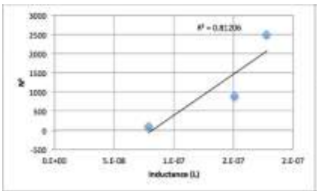
\includegraphics[scale=0.9]{inductance.png}
\end{figure}

The results of the Faraday effect were recorded in LabView software.\\

The Meissner effect results are plotted below.

\begin{figure}[h!]
\centering
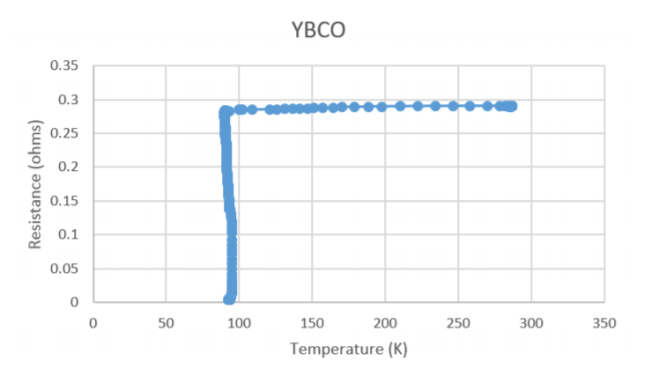
\includegraphics[scale=0.5]{meissner.png}
\end{figure}

\section{Observations}

Plotting Inductance vs N$^2$ while keeping a constant length and area will give a linear relationship by the equation below.
$$L = (\mu_r\mu_0N^2A)/L$$
We can see how the linearization of the data in the results confirms the equation.\\

The Faraday effect was observed to be greater with larger magnets, and greater with increasing velocity of the magnet. This confirms the equation we saw in class.\\

The Meissner effect was seen to occur, as we saw superconductivity occur once the material fell below a certain temperature. This also was visually observed as we saw flux pinning as we levitated a ferromagnet above the superconducting material.

\end{document}